\documentclass[12pt]{article}

\usepackage{amsmath, amssymb}
\usepackage{graphicx}
\usepackage{float}
\usepackage[margin=1in]{geometry}

\title{MA 550: Homework 1}
\author{Axel Fraud}
\date{}

\begin{document}

\maketitle

% ============================================================
% Problem 1
% ============================================================

\section*{Problem 1}

Consider the two-dimensional Stokes equations
\[
\mu \nabla^2 \mathbf{u} - \nabla P = \mathbf{b},
\qquad
\nabla \cdot \mathbf{u} = 0,
\]
where
\[
\mathbf{u} =
\begin{bmatrix}
U \\ V
\end{bmatrix},
\qquad
\mathbf{b} =
\begin{bmatrix}
f \\ g
\end{bmatrix},
\qquad
\mu = 1.
\]

The manufactured analytical solutions are
\[
U_{\mathrm{an}}(x,y)
=
\sin(2\pi y)\sin(2\pi x),
\]
\[
V_{\mathrm{an}}(x,y)
=
-3.5
+
\cos(2\pi x)
\left[\cos(2\pi y)-1\right],
\]
and
\[
P_{\mathrm{an}}(x,y)
=
\sin(2\pi y)\cos(2\pi x).
\]

The velocity and pressure are periodic on the left and right boundaries. On
the top and bottom boundaries,
\[
U=0,
\qquad
V=-3.5.
\]

\subsection*{Solution}

The Stokes equations were discretized on a MAC staggered grid. Pressure
unknowns were placed at cell centers, the horizontal velocity $U$ was placed
on vertical cell faces, and the vertical velocity $V$ was placed on horizontal
cell faces. This staggering allows the pressure gradients and velocity
divergence to be approximated naturally at their corresponding grid
locations.

Using second-order centered finite differences, the discrete Stokes system
was assembled in block form as
\[
\begin{bmatrix}
\mu L_U & 0 & -G_x \\
0 & \mu L_V & -G_y \\
D_x & D_y & 0
\end{bmatrix}
\begin{bmatrix}
U \\ V \\ P
\end{bmatrix}
=
\begin{bmatrix}
f_{\mathrm{bc}} \\
g_{\mathrm{bc}} \\
h_{\mathrm{bc}}
\end{bmatrix}.
\]

Here, $L_U$ and $L_V$ are the discrete Laplacian operators, $G_x$ and
$G_y$ are the discrete pressure-gradient operators, and $D_x$ and $D_y$
form the discrete divergence operator. Periodicity in the $x$-direction was
implemented directly through periodic indexing. The prescribed velocity
values on the top and bottom boundaries were incorporated into the
appropriate right-hand-side terms.

Since pressure in the Stokes equations is determined only up to an additive
constant, the discrete system contains a pressure null space. To obtain a
unique numerical solution, one pressure degree of freedom was fixed while
solving the linear system. After solving, the mean numerical pressure was
subtracted before comparison with the manufactured pressure:
\[
P_{\mathrm{num}}
\leftarrow
P_{\mathrm{num}}
-
\frac{1}{N_P}
\sum_{i=1}^{N_P} P_{\mathrm{num},i}.
\]

As a consistency check, the discrete gradient and divergence operators
satisfied
\[
\left\|G_x+D_x^T\right\|_{\max}=0,
\qquad
\left\|G_y+D_y^T\right\|_{\max}=0.
\]
This verifies the expected discrete adjoint relationship between the
gradient and divergence operators.

The computed velocity components had the ranges
\[
-0.998970 \leq U \leq 0.998970,
\]
and
\[
-5.497939 \leq V \leq -1.502061.
\]
The corresponding velocity magnitude satisfied
\[
1.508223
\leq
\|\mathbf{u}\|
\leq
5.491793.
\]

Because $U$ and $V$ are stored at different locations on the staggered grid,
the two components were interpolated to the pressure-cell centers before
computing the velocity magnitude and plotting the streamlines. The resulting
numerical velocity field is shown in Figure~\ref{fig:p1}.

\begin{figure}[H]
    \centering
    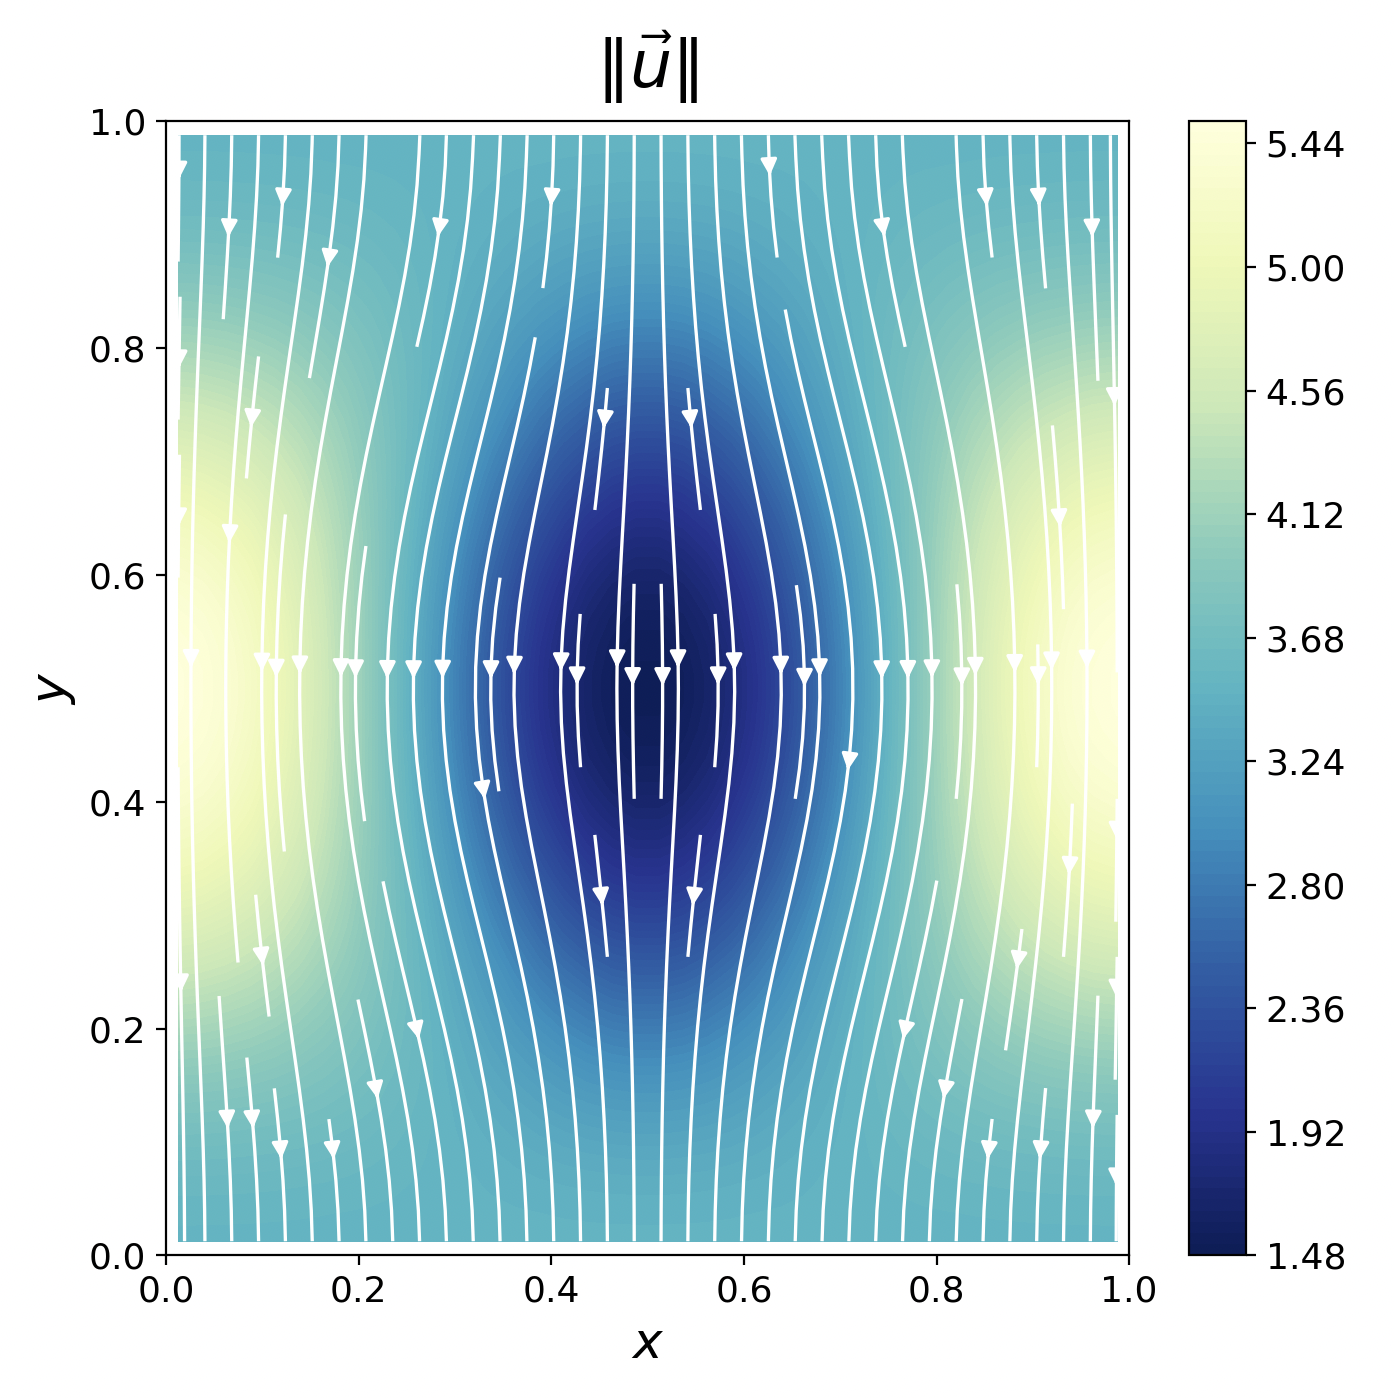
\includegraphics[width=0.68\textwidth]{P1}
    \caption{Numerical velocity magnitude and streamlines for the manufactured
    Stokes solution.}
    \label{fig:p1}
\end{figure}

The numerical solution agrees closely with the manufactured solution. The
maximum absolute errors were
\[
\max |U_{\mathrm{num}}-U_{\mathrm{an}}|
=
1.023963\times10^{-3},
\]
\[
\max |V_{\mathrm{num}}-V_{\mathrm{an}}|
=
3.076324\times10^{-3},
\]
and
\[
\max |P_{\mathrm{num}}-P_{\mathrm{an}}|
=
1.022491\times10^{-3}.
\]

The streamline pattern in Figure~\ref{fig:p1} is consistent with the
manufactured velocity field. The small errors in all three solution
variables, together with the operator consistency checks, indicate that the
staggered-grid Stokes discretization is correctly reproducing the analytical
solution.

% ============================================================
% Problem 2
% ============================================================

\section*{Problem 2}

Perform an error analysis by solving the Stokes system on increasingly fine
grids with
\[
N_x=N_y.
\]
For each grid, compute the relative $L^2$ error. For example, the error in
$U$ is defined by
\[
\mathrm{err}_U
=
\frac{
\|U_{\mathrm{num}}-U_{\mathrm{an}}\|_2
}{
\|U_{\mathrm{an}}\|_2
}.
\]
The same relative error was computed for $V$ and $P$. The goal is to
demonstrate second-order convergence as the grid is refined.

\subsection*{Solution}

The Stokes solver from Problem 1 was applied on a sequence of uniform grids
with
\[
N_x=N_y=N,
\]
where
\[
N=10,20,30,\ldots,100.
\]
For each grid resolution, the numerical velocity components were first
interpolated to the pressure-cell centers so that the numerical and
manufactured solutions were evaluated at the same spatial locations. As in
Problem 1, the mean of the numerical pressure was removed before computing
the pressure error.

The relative $L^2$ errors were calculated using
\[
E_U
=
\frac{
\|U_{\mathrm{num}}-U_{\mathrm{an}}\|_2
}{
\|U_{\mathrm{an}}\|_2
},
\qquad
E_V
=
\frac{
\|V_{\mathrm{num}}-V_{\mathrm{an}}\|_2
}{
\|V_{\mathrm{an}}\|_2
},
\]
and
\[
E_P
=
\frac{
\|P_{\mathrm{num}}-P_{\mathrm{an}}\|_2
}{
\|P_{\mathrm{an}}\|_2
}.
\]

To measure the observed convergence rate between consecutive grids, the
order was calculated from
\[
p
=
\frac{
\log(E_{N_1}/E_{N_2})
}{
\log(h_{N_1}/h_{N_2})
},
\qquad
h_N=\frac{1}{N}.
\]
For a second-order discretization, we expect
\[
E=\mathcal{O}(h^2),
\]
and therefore an observed convergence order approaching
\[
p=2.
\]

First- and second-order reference curves were also included in the
log--log error plot. The reference curves were scaled from the initial
$U$ error according to
\[
E_{\mathrm{first}}
=
E_U(10)
\left(\frac{10}{N}\right),
\]
and
\[
E_{\mathrm{second}}
=
E_U(10)
\left(\frac{10}{N}\right)^2.
\]

The resulting convergence behavior is shown in
Figure~\ref{fig:p2}.

\begin{figure}[H]
    \centering
    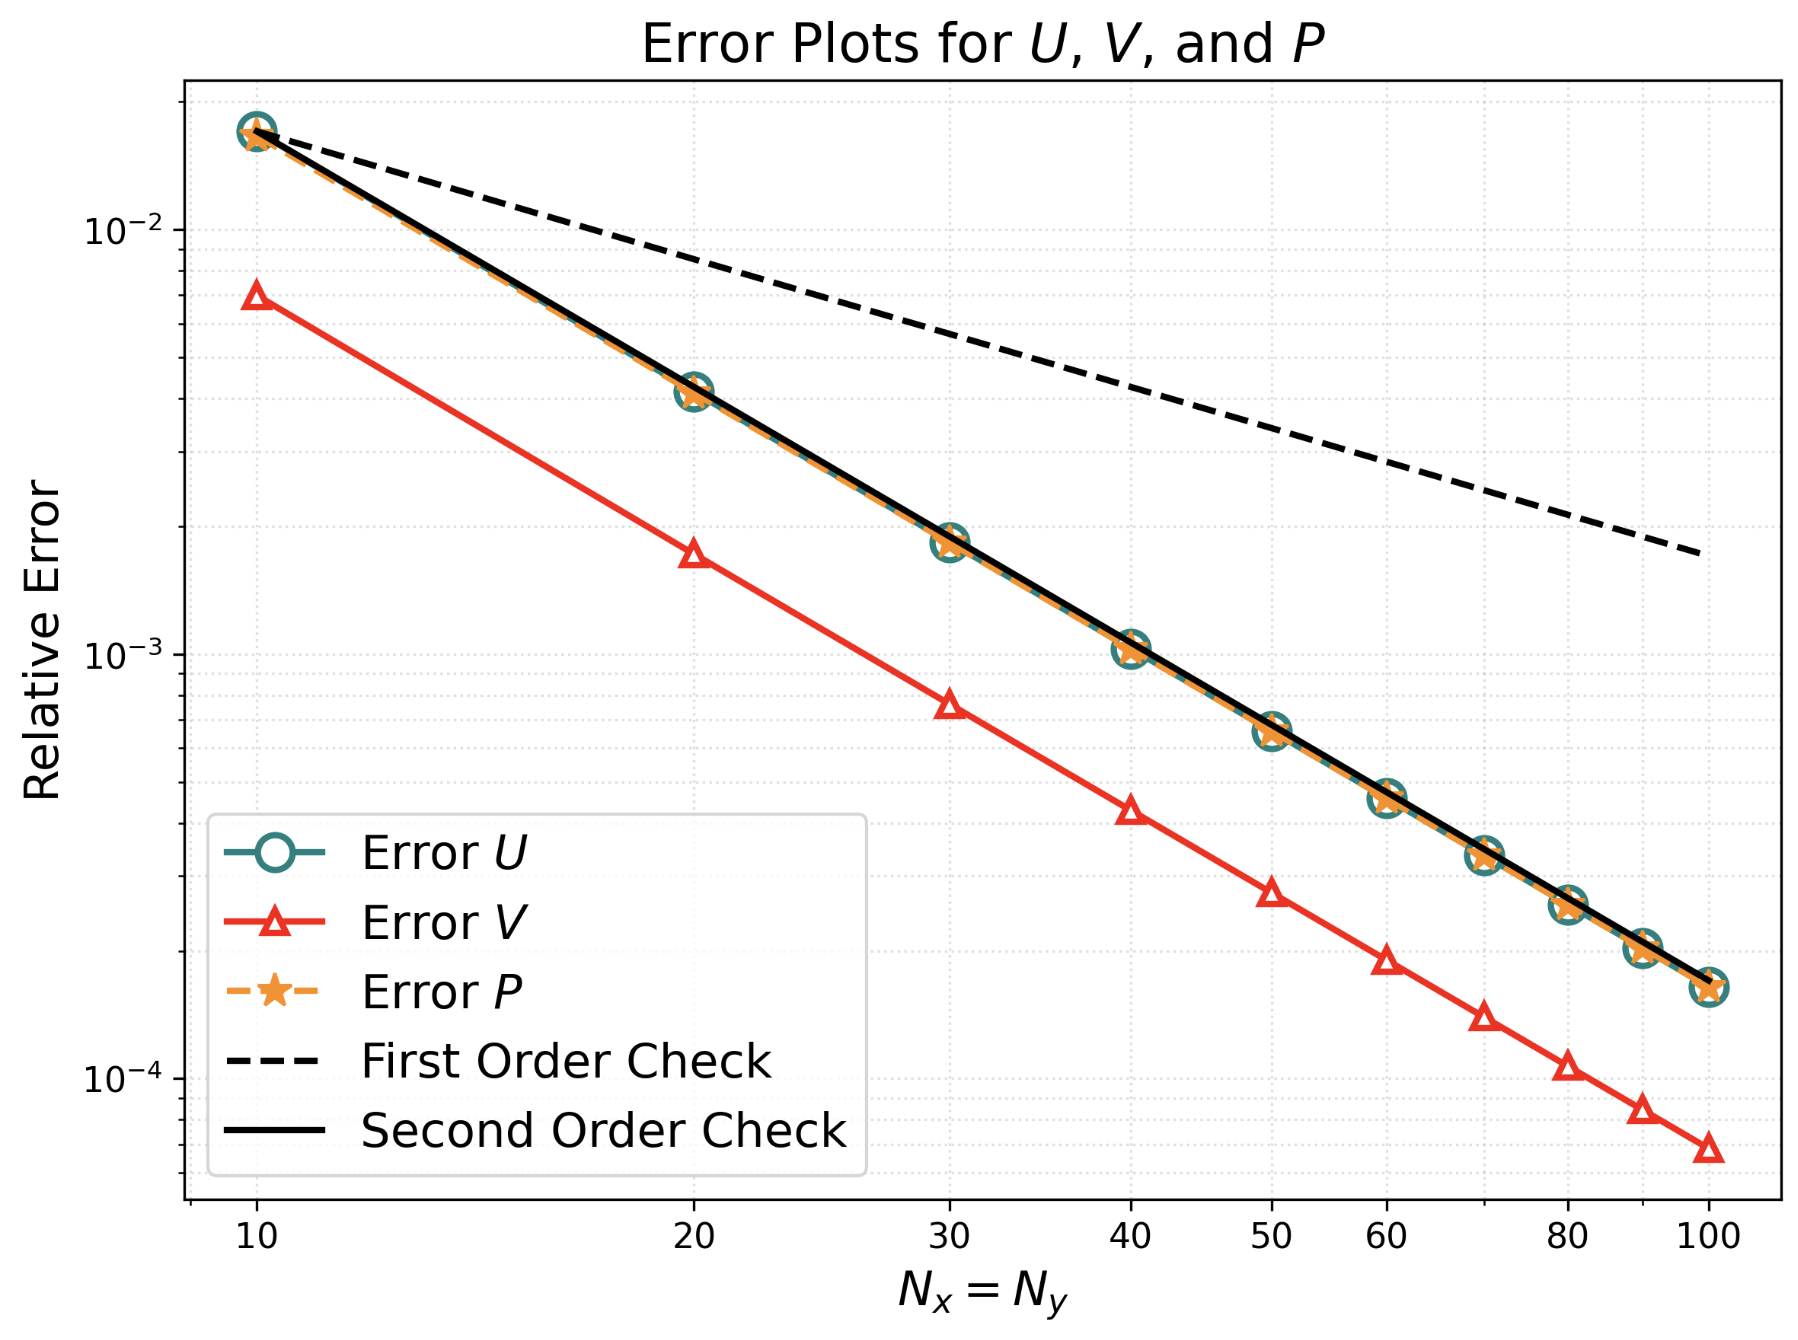
\includegraphics[width=0.82\textwidth]{P2}
    \caption{Relative $L^2$ errors for $U$, $V$, and $P$ under grid
    refinement, together with first- and second-order reference curves.}
    \label{fig:p2}
\end{figure}

As the grid is refined, the errors in all three solution variables decrease
consistently. The $U$ and $P$ errors are nearly identical over the tested
grid resolutions, which causes their curves to nearly overlap in
Figure~\ref{fig:p2}. The $V$ error is smaller in magnitude, but follows the
same convergence trend.

Most importantly, the numerical error curves are approximately parallel to
the second-order reference curve and decrease substantially faster than the
first-order reference curve. The observed orders provide a quantitative
confirmation of this behavior. For the initial refinement from $N=10$ to
$N=20$, the observed orders were
\[
p_U=2.0374,
\qquad
p_V=2.0233,
\qquad
p_P=2.0125.
\]
As the grid was refined, these values approached $2$. For the final
refinement from $N=90$ to $N=100$, the observed orders were
\[
p_U=2.0008,
\qquad
p_V=2.0005,
\qquad
p_P=2.0003.
\]
Therefore,
\[
E_U=\mathcal{O}(h^2),
\qquad
E_V=\mathcal{O}(h^2),
\qquad
E_P=\mathcal{O}(h^2).
\]
This demonstrates the expected second-order convergence of the staggered-grid
finite-difference discretization for the manufactured Stokes problem.

% ============================================================
% Problem 3
% ============================================================

\section*{Problem 3: Charlie's Rule}

For this problem, I chose to explore making the Stokes solver more flexible
by applying it to a different set of boundary conditions.

\subsection*{Lid-Driven Stokes Cavity}

Rather than using the periodic boundary conditions and manufactured solution
from Problems 1 and 2, I modified the solver to model a lid-driven cavity.
The computational domain remained the unit square,
\[
\Omega=[0,1]\times[0,1],
\]
and the governing equations remained
\[
\mu\nabla^2\mathbf{u}-\nabla P=\mathbf{0},
\qquad
\nabla\cdot\mathbf{u}=0,
\]
with
\[
\mu=1.
\]

The upper boundary of the cavity was prescribed to move horizontally with
unit velocity,
\[
U(x,1)=1,
\qquad
V(x,1)=0,
\]
while the remaining three walls were stationary with no-slip boundary
conditions,
\[
U=V=0.
\]

This creates a substantially different problem from the manufactured
solution used previously. In Problems 1 and 2, the left and right boundaries
were periodic and the forcing terms were constructed from a known analytical
solution. Here, there is no manufactured velocity field driving the solution.
Instead, the motion of the upper wall drives the flow inside the cavity.

\subsection*{Numerical Implementation}

I retained the MAC staggered-grid structure from the original Stokes solver,
with pressure at cell centers and the two velocity components located on
their corresponding cell faces. The main modification was the treatment of
the boundaries.

The periodic indexing used previously in the horizontal direction was
replaced by wall boundary conditions. The stationary left, right, and bottom
walls enforce zero velocity, while the upper wall imposes the nonzero
horizontal lid velocity. These prescribed values were incorporated into the
finite-difference equations through the boundary contributions to the
right-hand side.

The resulting discrete system retained the same general Stokes block
structure,
\[
\begin{bmatrix}
\mu L_U & 0 & -G_x \\
0 & \mu L_V & -G_y \\
D_x & D_y & 0
\end{bmatrix}
\begin{bmatrix}
U \\ V \\ P
\end{bmatrix}
=
\begin{bmatrix}
f_{\mathrm{bc}} \\
g_{\mathrm{bc}} \\
h_{\mathrm{bc}}
\end{bmatrix},
\]
but the operators and boundary contributions now correspond to the
nonperiodic cavity walls. As before, the pressure is determined only up to
an additive constant, so a pressure degree of freedom was fixed to remove
the null space.

After solving the system, the staggered velocity components were interpolated
to the pressure-cell centers. The velocity magnitude was then computed as
\[
\|\mathbf{u}\|
=
\sqrt{U^2+V^2}.
\]

Figure~\ref{fig:p3_velocity} shows the resulting velocity magnitude and
streamlines.

\begin{figure}[H]
    \centering
    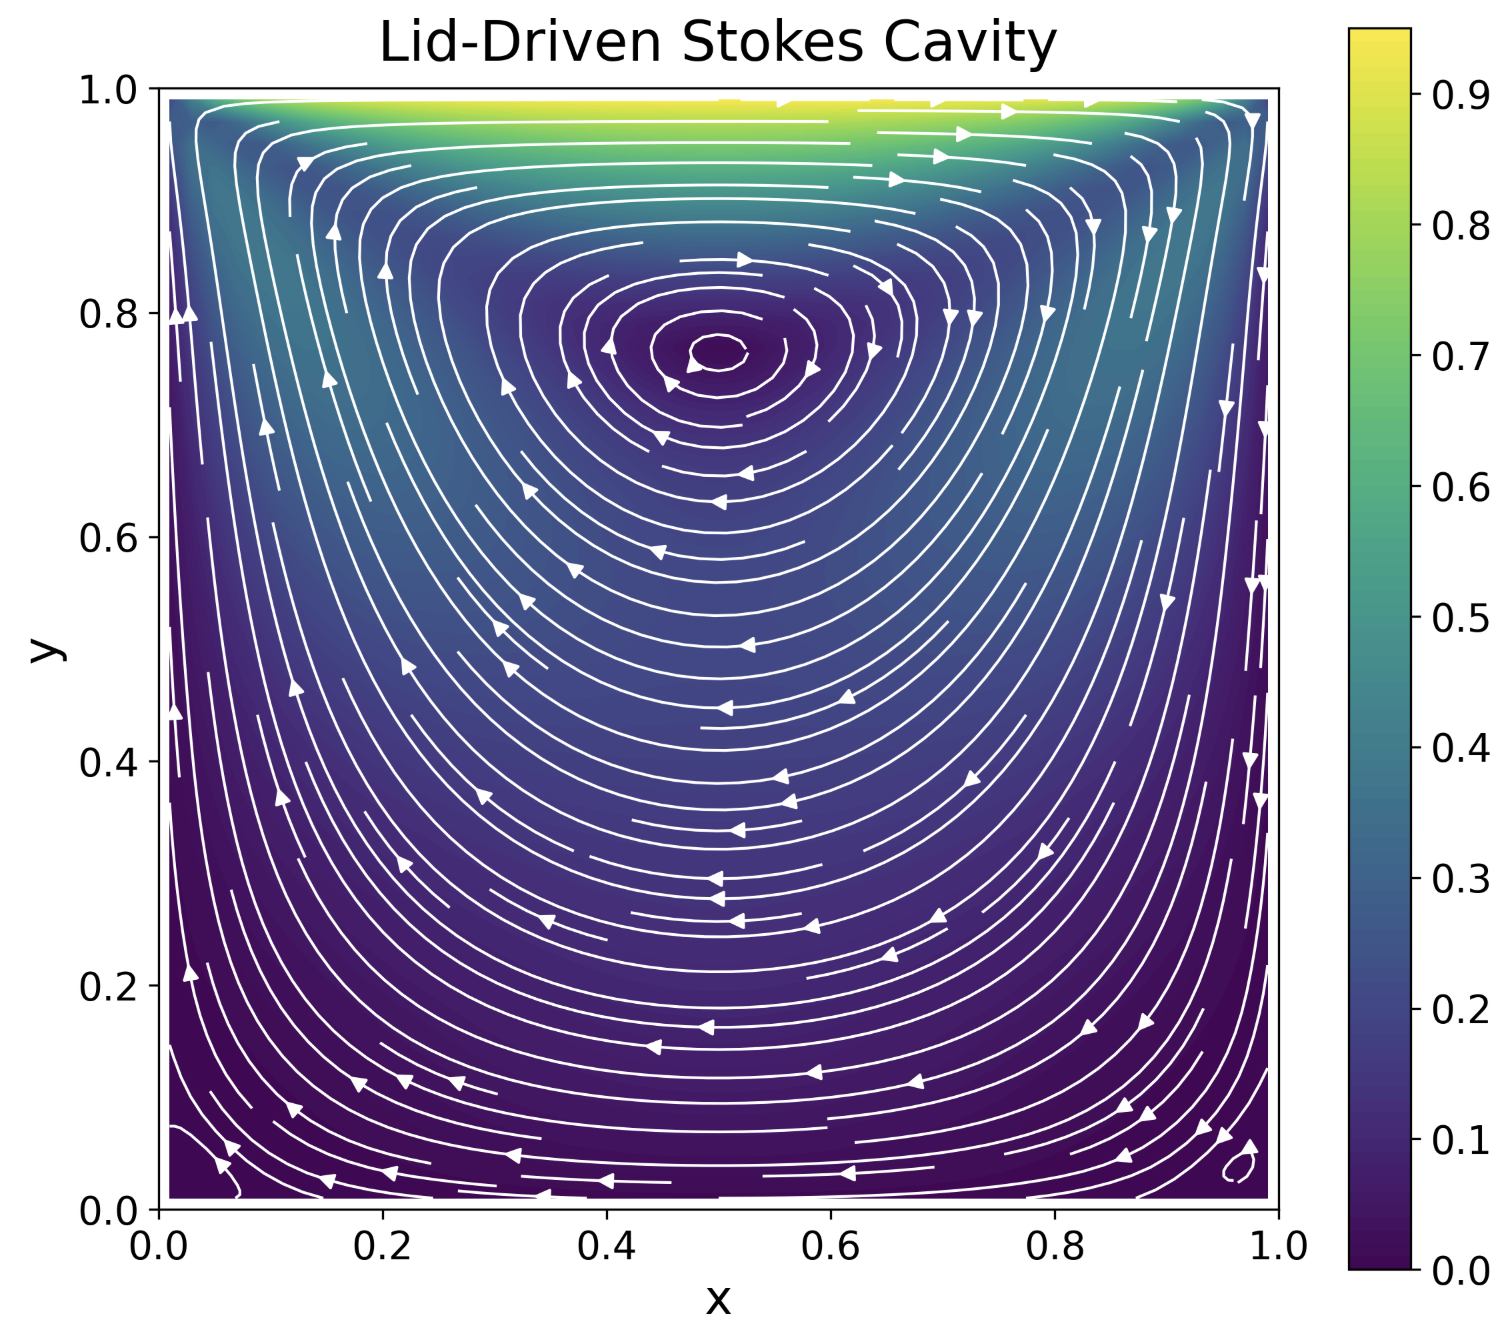
\includegraphics[width=0.70\textwidth]{P3_1}
    \caption{Velocity magnitude and streamlines for the lid-driven Stokes
    cavity.}
    \label{fig:p3_velocity}
\end{figure}

The effect of the moving upper wall is clearly visible. The largest velocity
magnitudes occur near the lid, where the prescribed horizontal velocity
directly drives the fluid. The motion of the lid produces a large clockwise
recirculation within the cavity. Moving away from the lid, the velocity
decreases as the flow approaches the stationary no-slip walls.

\subsection*{Vorticity}

To further explore the numerical solution, I also computed the two-dimensional
vorticity field. For a velocity field
\[
\mathbf{u}=(U,V),
\]
the scalar vorticity is
\[
\omega
=
\frac{\partial V}{\partial x}
-
\frac{\partial U}{\partial y}.
\]

The derivatives were approximated numerically from the cell-centered
velocity components. The resulting vorticity field is shown in
Figure~\ref{fig:p3_vorticity}. Streamlines are included again to show the
relationship between the rotational structure and the velocity field.

\begin{figure}[H]
    \centering
    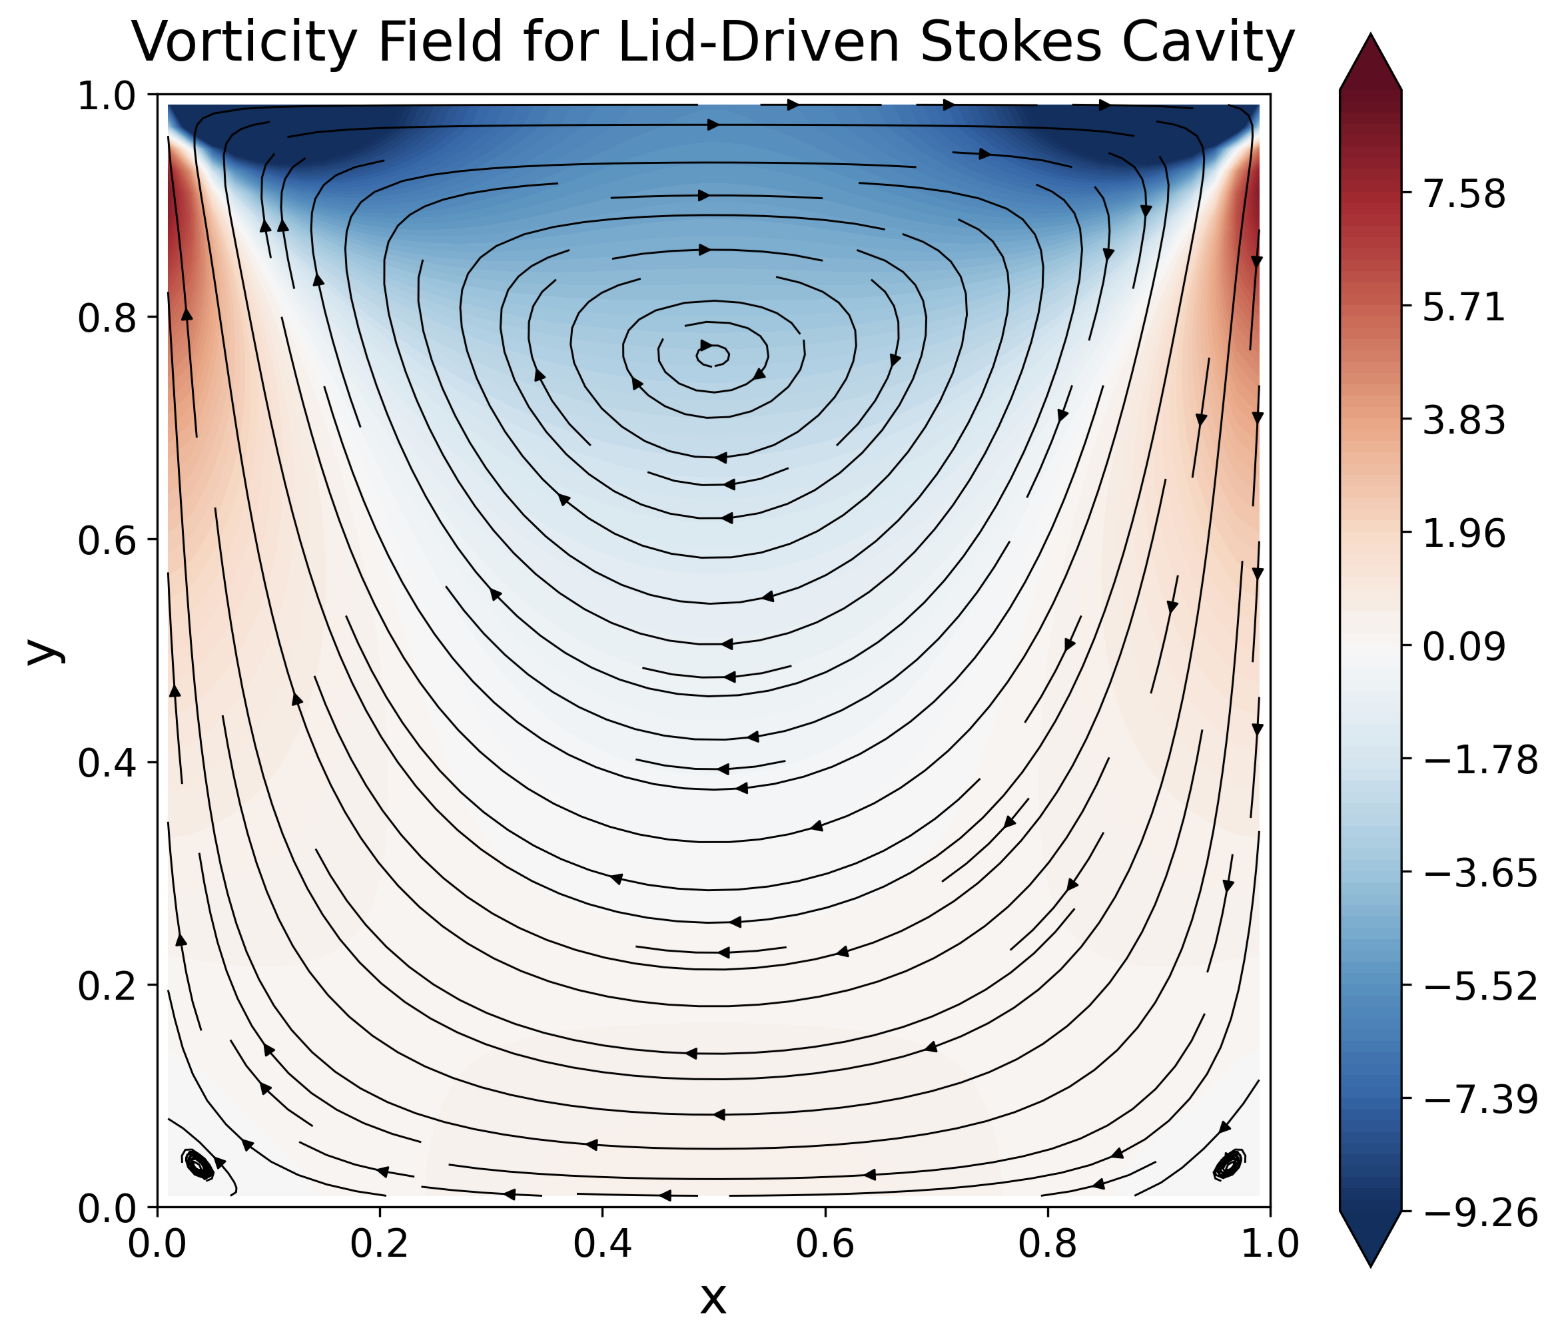
\includegraphics[width=0.70\textwidth]{P3_3}
    \caption{Vorticity field and streamlines for the lid-driven Stokes
    cavity.}
    \label{fig:p3_vorticity}
\end{figure}

The vorticity plot highlights behavior that is less apparent from the
velocity magnitude alone. Strong vorticity develops near the moving upper
wall because of the large velocity gradient between the moving lid and the
interior fluid. Strong variations also appear near the upper corners, where
the moving lid meets the stationary side walls. The interior streamline
pattern corresponds to the large clockwise recirculation observed in
Figure~\ref{fig:p3_velocity}.

\subsection*{Conclusion}

This experiment demonstrates that the staggered-grid Stokes solver is not
limited to the manufactured periodic problem used for verification in
Problems 1 and 2. By modifying the boundary treatment while retaining the
same underlying MAC-grid formulation, the solver can be applied to a
qualitatively different flow problem. The lid-driven cavity produces the
expected recirculating flow, and computing the vorticity provides an
additional way to investigate the structure of the numerical solution.

\end{document}